%%%%%%%%%%%%%%%%%%%%%%%%%%%%%%%%%%%%%%%%%%%%%%%%%%%%%%%%%%%%%%%%%%%%%%%%%%%%%%%%
\documentclass[11pt]{article}
\pagenumbering{arabic}
%%%%%%%%%%%%%%%%%%%%%%%%%%%%%%%%%%%%%%%%%%%%%%%%%%%%%%%%%%%%%%%%%%%%%%%%%%%%%%%%

%%%%%%%%%%%%%%%%%%%%%%%%%%%%%%%%%%%%%%%%%%%%%%%%%%%%%%%%%%%%%%%%%%%%%%%%%%%%%%%%
\usepackage{amsmath}
\usepackage[pdftex]{graphicx}
\usepackage{color}
\usepackage{subfigure}
\usepackage{enumitem}
\usepackage{sidecap}

%%%%%%%%%%%%%%%%%%%%%%%%%%%%%%%%%%%%%%%%%%%%%%%%%%%%%%%%%%%%%%%%%%%%%%%%%%%%%%%%
\hsize=6.5in
\hoffset=-0.75in
\setlength{\textwidth}{6.5in}
\setlength{\textheight}{9in}
\setlength{\voffset}{0pt}
\setlength{\topmargin}{0pt}
\setlength{\headheight}{0pt}
\setlength{\headsep}{0pt}

\vsize=9.0in
\renewcommand\baselinestretch{0.93}
%%%%%%%%%%%%%%%%%%%%%%%%%%%%%%%%%%%%%%%%%%%%%%%%%%%%%%%%%%%%%%%%%%%%%%%%%%%%%%%%

\normalsize

%%%%%%%%%%%%%%%%%%%%%%%%%%%%%%%%%%%%%%%%%%%%%%%%%%%%%%%%%%%%%%%%%%%%%%%%%%%%%%%
\usepackage{hyperref}
\hypersetup{
    colorlinks=true,   % false: boxed links; true: colored links
    linkcolor=red,     % color of internal links
    citecolor=red,     % color of links to bibliography
    filecolor=magenta, % color of file links
    urlcolor=blue      % color of external links
}
%%%%%%%%%%%%%%%%%%%%%%%%%%%%%%%%%%%%%%%%%%%%%%%%%%%%%%%%%%%%%%%%%%%%%%%%%%%%%%%

%%%%%%%%%%%%%%%%%%%%%%%%%%%%%%%%%%%%%%%%%%%%%%%%%%%%%%%%%%%%%%%%%%%%%%%%%%%%%%%%
%%%%%%%%%%%%%%%%%%%%%%%%%%%%%%%%%%%%%%%%%%%%%%%%%%%%%%%%%%%%%%%%%%%%%%%%%%%%%%%%
\begin{document}

%%%%%%%%%%%%%%%%%%%%%%%%%%%%%%%%%%%%%%%%%%%%%%%%%%%
\centerline{\Large\bf RUI Impact Statement}
\vspace{0.2cm}
%%%%%%%%%%%%%%%%%%%%%%%%%%%%%%%%%%%%%%%%%%%%%%%%%%%

%%%%%%%%%%%%%%%%%%%%%%%%%%%%%%%%%%%%%%%%%%%%%%%%%%%
\section{Siena College}
%%%%%%%%%%%%%%%%%%%%%%%%%%%%%%%%%%%%%%%%%%%%%%%%%%%
Siena College, founded in 1937, is a coeducational, independent, liberal arts college 
with a Franciscan tradition that serves approximately 3400 students. It is located in Loudonville, New York,
in the center of New York State's Capital District.

Siena College provides a unique array of outstanding scientific, reference, and research facilities
for a small liberal arts college. Recently, the College opened the J. Spencer and Patricia Standish
Library. This 72,000 square foot building provides access to 100 computer workstations, 
500 Internet connections, a computer laboratory, and a 40-seat screening room. Moreover, with Rensselaer
Polytechnic Institute (RPI) and the State University of New York at Albany nearby, there is further
access to first-rate research libraries via a collaborative exchange agreement with Siena. The
Morrell Science Center, opened in September 2001, is a 55,000 square foot science center with 24
research labs, 10 teaching labs, and three support areas on three floors. 
Siena has recently (Summer 2014) completed the construction of the
Stewarts Advanced Instrumentation \& Technology (SAInT) Center with the goal of
establishing Siena as a leader in undergraduate education in scientific
instrumental resources and training. 
and it houses multiple mass spectrometers,
an atomic force microscope, a scanning electron microscope, and other
analytic equipment.  Electronics, machine shops, and a
High Performance Computing Center are also available for science/research support.

The administration at Siena College is fully supportive of faculty research efforts, willingly reducing
the normal teaching load from 12 to 9 contact hours per semester for faculty actively pursuing
research. The Physics department chair is proactive in creatively balancing the
teaching load for faculty who are conducting grant-supported research.
%The administration is supportive of an additional course reduction to 6 contact hours
%per semester if the faculty member can secure outside funding.

Over the past several years, Siena College has undergone an academic transformation in
response to its exponential growth in sponsored research grants (see Graph 1) and faculty-student
collaborations. 
As of this fall, there are active grants in the School of Science totaling \$6.5M,
and integrated over the last 10 years, the faculty have brought in a sum total
of \$12.5M. 
A significant number of students are engaged in a research
project under the supervision of a faculty member are funded by federal sponsors committed to
advancing the sciences (i.e., NSF, NASA). During the summer months, a large cohort of
students from across all disciplines participates in undergraduate research as part of the 
{\it Siena Summer Scholars Program}.

To ensure adequate oversight, management and recognition of all
faculty-student collaborative activities, in fall 2008 the college
established the {\it Center for Undergraduate Research and Creative
Activities (CURCA)}. The mission of CURCA is to foster a campus-
wide culture in which all undergraduates are engaged in inquiry or
investigations conducted in collaboration with a faculty mentor that
makes an original intellectual or creative contribution to a
discipline or the community. The overarching goal of CURCA is
to afford students an undergraduate research experience to work
collaboratively with a faculty mentor on a creative, original project.
In addition, the college provides well-structured undergraduate
research experience that will lead to increased student engagement
and preparation for post-baccalaureate opportunities upon
graduation. In 2011, CURCA was endowed with a \$1.5
million gift to ensure long-term success and sustainability.
Since the creation of CURCA, the number of faculty-collaborations
has grown steadily.  Since 2008, the number of students participating
in an undergraduate research experience has more than tripled. 
%As of 2008 to the present, the number of
%students participating in an undergraduate research experience
%more than tripled from 20 to 76 students (see Table.~\ref{tab:curca0}). 
%This represents a 74\%
%growth in undergraduate research participation by students over a
%five year period (see Table 1 for additional information). 
To ensure day to day management and
oversight of CURCA on a full-time basis, the college appointed its first undergraduate research
director on June 1, 2012.

%\begin{table}[h]
    %\caption{Student Participation in Undergraduate Research Activities, 2008 - present.\label{tab:curca0}}
    %\begin{tabular}{c c c c c}
    %\hline
    %& {\bf Students on Sponsored} & {\bf Students on Sponsored} &   &  \\
     %& {\bf Funded Projects} & {\bf Funded Projects} & {\bf Siena College}  &   \\
    %{\bf Year} & {\bf (Academic Year)} & {\bf (Summer)} & {\bf Summer Scholars}  &  {\bf Total} \\
%\hline
%2007 &6 &5 &8 &20 \\
%2008 &9 &15&28&52 \\
%2009 &15&20&19&54 \\
%2010 &16&28&28&72 \\
%2011 &17&28&37&82 \\
%2012 &11&24&41&76 \\
%\end{tabular}
%\end{table}

\begin{SCfigure}
    \centering
    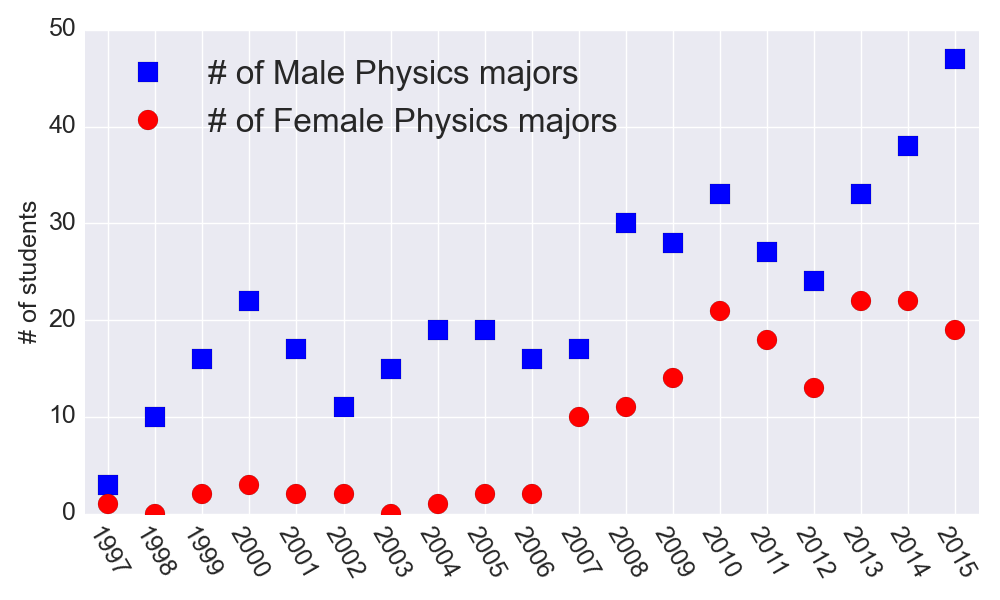
\includegraphics[height=0.25\textheight]{figures/dept_plot.png}
    \caption{The growth of the Physics department, particularly
        among women, has been striking over the last 10 years. 
        This is due in part to the high-level of engagement that the faculty
        have in involving students in research projects and in proactively
        recruiting and retaining young women scientists.
     \label{fig:dept}}
\end{SCfigure}

%%%%%%%%%%%%%%%%%%%%%%%%%%%%%%%%%%%%%%%%%%%%%%%%%%%%%%%%%%%%%%%%%%%%%%%%%%%%%%%%
\section{Siena College Physics \& Astronomy Program}
%%%%%%%%%%%%%%%%%%%%%%%%%%%%%%%%%%%%%%%%%%%%%%%%%%%%%%%%%%%%%%%%%%%%%%%%%%%%%%%%
The Department of Physics aims to develop in its students a comprehensive grasp of the principles of physics. The program
emphasizes the concepts and techniques that have led to our present state of understanding of
the physical universe. Placed in the context of a liberal arts environment, the generality and
applicability of the physics curriculum give physics majors three broad options upon graduation.
He or she is well prepared to pursue graduate study in physics or a related field, to embark
immediately upon a professional career in science, or to enter one of the numerous careers which
require or are enhanced by a broad knowledge of science in today's technological society.

A curriculum is offered for those interested in teaching, and the department also offers a 3/2 Engineering
program in affiliation with Clarkson University, Rensselaer Polytechnic Institute (RPI),
and Binghamton University leading to a B.S. in Physics and a
B.E. in electrical, mechanical, civil, biomedical, aeronautical, nuclear or materials engineering.
Programs leading to a Master's degree are also available through RPI and Union Graduate College.

Siena is a small liberal arts college that emphasizes teaching excellence, small class sizes and close 
student-faculty connections.  Unlike many comparable schools, Siena's Department of Physics \&
Astronomy at Siena also has a very strong research program with many federally funded projects.  
%The Dean of our School of Science, Dr. Allan Weatherwax, leads a collaboration that has been awarded 
%several large NSF grants (totaling over four million dollars) to extend their work on terrestrial and 
%planetary plasmas (e.g. NSF ANT awards 0840158, 0638587 and AGS Awards 0838015, 0753840 and 0753451).  
Dr. John Cummings, the current Dean of Science, is funded by the NSF to work on 
neutrino physics at Daya Bay, China (NSF PHY-0901954).  Dr. Rose Finn is an 
NSF Career Fellow (Award 0847430) and has funding through the Spitzer Space Telescope Observer program, 
and Dr. Tom Coohill is funded through the Department of Defense.  Dr. John Moustakas
has recieved multiple grants for viewing time on the Hubble Space Telescope. Drs. Larry Medsker, Rose Finn, and 
Allan Weatherwax share an NSF S-STEM grant (DUE 0728452) and Dr. Medsker and Dr. Michele McColgan share 
an NSF Robert Noyce Teacher Scholarship Program grant (DUE-1136322). Drs. Finn and Medsker recently 
completed a Clare Boothe Luce grant that provided scholarships for women majoring in STEM areas. 
 
The Department of Physics \& Astronomy is experiencing an exciting
period of growth and revitalization with 5 new faculty members in the
last 7 years.  The number of physics majors has grown as well, and we
are particularly proud of the recent increase in the number of women
physics majors! (see Fig.~\ref{fig:dept})
The strength of our research program reflects a dramatic transformation of the department over the 
past decade, accomplished through a focused emphasis on excellence in STEM education supported by 
faculty research that integrates undergraduates in ways that enable them to make meaningful contributions 
to the field.  These changes have enhanced our ability to recruit new students and the number of 
physics majors increased from an average of 16 between 1997 and 2006 to 66 in 2015. The number of 
female majors increased from an average of 1.5 to about 20 over that same time period.
%\textcolor{red}{Can we say something here about the number of students in the department participating in 
%undergraduate research and perhaps some specific examples?  Also something about post-graduate placement and employment?}
 
The transformation of Physics \& Astronomy at Siena College is a testament to strategic vision, research-intensive 
faculty who love teaching, a focus on undergraduate research, and the critical
importance of NSF funding for basic research and undergraduate STEM education. 
%The requested funding will help us...

%%%%%%%%%%%%%%%%%%%%%%%%%%%%%%%%%%%%%%%%%%%%%%%%%%%%%%%%%%%%%%%%%%%%%%%%%%%%%%%%
\section{Impact of this proposal}
%%%%%%%%%%%%%%%%%%%%%%%%%%%%%%%%%%%%%%%%%%%%%%%%%%%%%%%%%%%%%%%%%%%%%%%%%%%%%%%% 
The PI is the only high energy particle physicist at Siena College. This grant
provides for a research program on the Compact Muon Solenoid (CMS) experiment at
the Large Hadron Collider (LHC) at CERN, one of the premier experiments
in particle physics. It is this type of large-scale, fundamental 
research that excites undergraduate students and entices them to study 
physics and related fields.

Through the support of this grant, undergraduate students will have many important
opportunities not normally available to a student at a liberal arts college.
\begin{itemize}[itemsep=0pt,parsep=0pt,topsep=0pt,partopsep=0pt]
    \item They will contribute to searches for new physics in some of the largest
        and most complex scientific experiments on the planet.
        Along the way, they will learn how nature works on a fundamental
        level.
    \item They will learn valuable skills such as computer programming (mostly
        in Python), data analysis, and statistical techniques.
    \item Siena students will travel to Cornell University, a top research university,
        and interact with the graduate students and post-docs there.
        This will motivate some of them to pursue graduate studies,
        when previously they might not have.
    \item Some select students will travel to Fermilab, the flagship national lab in the US for particle
        physics. 
    \item Some will also have the opportunity to travel overseas to CERN, the site
        of the LHC and some of the most exciting scientific research in the world.
    \item Students will learn about how large international scientific collaborations function.
    \item Students will have the opportunity to be a co-author on a paper and present their
        work at professional meetings.
\end{itemize}

Students supported by this grant will move on to the next phase of their careers more prepared for scientific and technological challenges.  Whether they pursue particle physics in graduate school or move on to industry, they will have learned valuable lessons in experimental problem solving.


%%%%%%%%%%%%%%%%%%%%%%%%%%%%%%%%%%%%%%%%%%%%%%%%%%%%%%%%%%%%%%%%%%%%%%%%%%%%%%%
\end{document}
%%%%%%%%%%%%%%%%%%%%%%%%%%%%%%%%%%%%%%%%%%%%%%%%%%%%%%%%%%%%%%%%%%%%%%%%%%%%%%%
